 \documentclass[12pt]{article}
%\usepackage[portuguese]{babel}
\usepackage{natbib}
\usepackage{url}
\usepackage[utf8x]{inputenc}
\usepackage{amsmath}
\usepackage{graphicx}
\graphicspath{{images/}}
\usepackage{parskip}
\usepackage{fancyhdr}
\usepackage{vmargin}
\setmarginsrb{1.5 cm}{2.5 cm}{1.5 cm}{2.5 cm}{1 cm}{1.5 cm}{1 cm}{1.5 cm}
\usepackage{hyperref}
\hypersetup{
    colorlinks=true,
    citecolor=black,
    filecolor=black,
    linkcolor=black,
    urlcolor=black
}
\let\oldhref\href
\renewcommand{\href}[2]{\oldhref{#1}{\bfseries#2}}

\usepackage[bottom]{footmisc}
\usepackage{caption}
\DeclareCaptionFormat{sanslabel}{#3}%
\usepackage[section]{placeins}
\usepackage{xcolor}
\definecolor{light-gray}{gray}{0.95}
\usepackage{listings}
\lstset{basicstyle=\ttfamily,
  showstringspaces=false,
  commentstyle=\color{red},
  keywordstyle=\color{blue},
  backgroundcolor=\color{light-gray},
  breaklines=true,
  extendedchars=true,
  basicstyle=\small,
  literate={é}{{\'e}}1
}
\lstset{aboveskip=15pt,belowskip=15pt}
\usepackage[autostyle]{csquotes}  
\def\labelitemi{--}
\usepackage{enumitem}
\setlist{nosep}
\usepackage{booktabs}

\title{Tutorial git}								% Title
%\author{}								% Author
\date{\today}											% Date

\makeatletter
\let\thetitle\@title
%\let\theauthor\@author
\let\thedate\@date
\makeatother

\pagestyle{fancy}
\fancyhf{}
%\rhead{\theauthor}
\lhead{\thetitle}
\cfoot{\thepage}

\begin{document}

%%%%%%%%%%%%%%%%%%%%%%%%%%%%%%%%%%%%%%%%%%%%%%%%%%%%%%%%%%%%%%%%%%%%%%%%%%%%%%%%%%%%%%%%%

\begin{titlepage}
	\centering
    \vspace*{0.5 cm}
    
\includegraphics[scale = 0.3]{resources/logo4.png}\\[1.0 cm]
    \textsc{\LARGE \newline\newline UNIX 101}\\[2.0 cm]
	\textsc{\Large or "How to feel like a true hack3r"}\\[0.5 cm]
	\rule{\linewidth}{0.2 mm} \\[0.4 cm]
	{ \huge \bfseries \thetitle}\\
	\rule{\linewidth}{0.2 mm} \\[1.5 cm]
	
%	\begin{minipage}{0.5\textwidth}
%		\begin{flushleft} \large
%			\emph{Professor:}\\
%			Renan E P Lima\\
%            Departamento de Matemática\\
%			\end{flushleft}
%			\end{minipage}~
%			\begin{minipage}{0.4\textwidth}
%           
%			\begin{flushright} \large
%			\emph{Grupo:} \\
%			Gabriel P Crestani\\
%           Victor R Sales\\
%		\end{flushright}
%        
%	\end{minipage}\\[2 cm]
	
	
    \thedate
    
    
    
	
\end{titlepage}

%%%%%%%%%%%%%%%%%%%%%%%%%%%%%%%%%%%%%%%%%%%%%%%%%%%%%%%%%%%%%%%%%%%%%%%%%%%%%%%%%%%%%%%%%

\tableofcontents
\pagebreak

%%%%%%%%%%%%%%%%%%%%%%%%%%%%%%%%%%%%%%%%%%%%%%%%%%%%%%%%%%%%%%%%%%%%%%%%%%%%%%%%%%%%%%%%%

\section{Foreword}

\subsection{Objective}
This tutorial should teach you the basics of working with git.
It will demonstrate what one can perform with this tool, how it works and how to use it.

If you work thoroughfully, at the end of this tutorial, you should know:

\begin{itemize}
\item What is git
\item Why it is important to know how to use git
%\item How to generate a SSH key and how to use SSH to communicate with a git server
\item How to clone a remote repository
\item How to contribute to a repository
\end{itemize}


\subsection{Preliminary setup}

You are going to need a UNIX-like operating system for this tutorial.
A Linux distribution is preferred but a Mac can also do the job (OS X is a variant of FreeBSD).

You also need the git binary to be installed on your system. If you have finished the first tutorial, you should know how to install it\footnote{Check that it is installed with \texttt{which git}; if it is not, install it with \texttt{sudo apt install git}. If you had trouble with that, take some time to read again the previous tutorial}.


\section{Git}

\subsection{The why: problems, problems, problems}

Because a coding project contains a lot of files of different type (code files, generated files, libraries, documentation, etc), working alone or collaborating on one proves itself to be complicated without some kind of versioning or collaboration tool.

Imagine having to share your work with colleagues throught USB keys or some cloud drive drag\&drop operations. Then imagine working all at the same time on the same project. How to handle conflicts? Regressions? What if your somehow loose your work? How do you restore it?

These problems can arise with a team of one or two persons and it is already a pain. Now imagine the same problems for a team of ten (or more) persons working on the same project. That is \textbf{a lot} of pain.

\subsection{The what: Version Control System}

Hopefully, smart people have worked on that problem for us, years ago. Version Control Systems (VCS) help solve some of these issues. There exist multiple VCS but \href{https://git-scm.com/}{git} is the most popular. Git is basically a tool that allows one to keep an history of files. It has the particularity to be distributed: multiple persons can keep a common history of files.

Thanks to git, you will be able to:

\begin{itemize}
\item Backup easily and whenever you want your work
\item Prevent accidents (e.g. unwanted file or content deletion)
\item Browse the history of your modifications and come back to some point in time if necessary
\item Work collaboratively on a project
\item ...and much more!
\end{itemize}


\subsection{The why you should really really learn using git}

Just to highlight the popularity of these kind of tools, one needs to understand that \textbf{every serious software company in the world use a VCS} and most of them rely on git.

It has been created for the needs of developing the Linux kernel and has quickly become a standard in the industry. It is a core tool for any professional worker in information systems : code is everywhere and versioning it is mandatory for systems to keep working continuously. Even infrastructure configurations are versioned now.

What is more, platforms like Github and Gitlab are rapidly raising in popularity. They provide developer/management tools on top of git: project management, automatic deployments, ticketing, etc. Most engineering teams use them on a daily basis.
These are widely used by companies and individuals all around the world. For this tutorial, we are going to use Github.%, Gitea, hosted on a dedicated server.

\section{Theory}

This tutorial is only going to cover the very basics of git. It has dozens of hidden features and it takes years to completely master that tool.

\subsection{Basics \& vocabulary}

The main goal of git is to allow one to \textit{versionate} files. That is done by keeping track of their history. The history of a file at some point in time could be pictured as the incremental changes made to it.

Let's take an example: a journalist writing a blog article on a word processor software (say Microsoft Word or Google Docs). First, he will start by writing the summary of the article in a document. That is \textit{"version 1"} of the file. Then, he will write down ideas, insights or some sentences. That is \textit{"version 2"}. Then, complete paragraphs. That makes it \textit{"version 3"}. Then, \textit{"version 4"} is the same thing with images and formatted text. Every logical change creates a new version of the document. The software keeps track of all of the versions; that is its \textbf{history}.

Git allows one to do exactly that for code directories. It keeps track of the history of multiple files at the same time (at a directory level), collaboratively.
The changes from one version to another are contained in what is called a \textbf{commit}. The project in which the files tracked by git are located is called a \textbf{repository}. The history of commits is called an... history. Lastly, although we are not going to cover them in this tutorial, parallel, alternative versions of a repository are called \textbf{branches}.

\subsection{State of files}

Git does not perform anything automatically. The user has to explicitely tell it what files should be tracked and how the history is going to be built. One interacts with git through the command line\footnote{There exists GUIs too but knowing the CLI is needed for most work environments :)}.

\begin{itemize}
\item Files that are not known by git are \textbf{untracked}
\item Files that are known by git but have not been modified are \textbf{unmodified}
\item Files that are known by git but have been modified are \textbf{modified} (or \textbf{unstaged})
\item Files that are known by git, have been modified and ready to be commited are \textbf{staged}
\end{itemize}

\subsection{Workflow}

In practice, to create an history for a project, the user simply changes the state of the files as he creates content. He can record changes to the repository through \textbf{commits}.

In modern software, generally, a new feature is all bundled in a \textbf{commit}. Then, each commit is more or less a logical change to the application. This is useful for many reasons. Here are two that I can think of from the top of my head:
\begin{itemize}
	\item At any moment, it makes it easy to look back in time and see when a feature has been implemented by checking the commit date associated with the feature
	\item If a newly coded feature introduces a bug in the application, one can revert the commit. This undoes the code changes introduced by the commit while a bugfix can be safely developed
\end{itemize}

\subsubsection{Basic commands}

The following commands can initialize a git repository
\begin{itemize}
\item \texttt{git init}: initialize an empty git repository in the working directory
\item \texttt{git clone remote\_path}: download a git repository from a remote place
\end{itemize}

The following commands can change the state of files in a git repository:
\begin{itemize}
\item \texttt{git add filename...}: add file named \texttt{filename} to commit if it is untracked. Only adds what changed since the previous version of that file if it is already tracked
\item \texttt{git commit [-m commit\_message]}: record staged files in a commit (with an optional commit message)
\item \texttt{git restore --staged file}: unstage file
\item \texttt{git checkout file}: erase changes made to file since last commit\footnote{Useful when deleting stuff by mistake!}
\item \texttt{git checkout commit|branch]}: "view" the state of the repository at some point of the history
\end{itemize}

The following commands help knowing the current state of a git repository:
\begin{itemize}
\item \texttt{git status}: show the working tree\footnote{The tree is the repository. Considering that there can be multiple branches in the history, if a commit is a node, we have a tree} status
\item \texttt{git log}: show the repository history
\item \texttt{git diff}: show changes between current state of files and last registered commit
\end{itemize}


\subsubsection{So, how to commit?}

The following snippets show an example of a simple git workflow. Read them carefully, then execute them on your workstation.

\begin{lstlisting}[language=bash]
$mkdir my_project # Creating a new directory
$cd my_project/ # Hopping inside...
$git init # Initializing a git repository in here
Initialized empty Git repository in /tmp/my_project/.git/ # It worked!
$touch my_code_file.py # Creating an empty file
$git status # Showing the current state of the tree
On branch master # Do not bother understanding branches right now

No commits yet # Makes sense, this is a new repository and we did not commit anything yet

Untracked files:
  (use "git add <file>..." to include in what will be committed)
	my_code_file.py # This file is not known by git: it is untracked

nothing added to commit but untracked files present (use "git add" to track)
$git add my_code_file.py # Staging this file (= preparing to put it in a future commit)
$git status # Showing the current state of the tree
On branch master

No commits yet

Changes to be committed:
  (use "git rm --cached <file>..." to unstage)
	new file:   my_code_file.py # Our file has correctly been staged! Our commit is now ready to be made :)


$git commit -m "Add code file with nothing inside" # Let's make a commit with our little file now
[master (root-commit) 33df133] Add code file with nothing inside # Done :)
 1 file changed, 0 insertions(+), 0 deletions(-)
 create mode 100644 my_code_file.py
$git status # Showing the current state of the tree
On branch master
nothing to commit, working tree clean # Indeed, we commited every change we made. No file has been modified since the last commit so everything is up-to-date.
$git log --oneline # Let us check the history
33df133 (HEAD -> master) Add code file with nothing inside # Our commit is just there. If we continue adding or modifying files and comitting them, we will have an history of all of our commits :)
\end{lstlisting}

We just initialized a git repository and made a commit with an empty file. Now let us say we modified the file and added some code inside. Let us see how to backup our work in a new commit.

\begin{lstlisting}[language=bash]
$cat my_code_file.py # Show content of the file
def power_2(x):
    return x * x
$git status # Showing the current state of the tree
On branch master
Changes not staged for commit:
  (use "git add <file>..." to update what will be committed)
  (use "git restore <file>..." to discard changes in working directory)
	modified:   my_code_file.py # That file is tracked by git but has been modified. In the previous example, it was not tracked by git at all so its label was "new file", not "modified"

no changes added to commit (use "git add" and/or "git commit -a")
$git diff # Let us see what has changed since last commit
diff --git a/my_code_file.py b/my_code_file.py
index e69de29..5dbce8e 100644
--- a/my_code_file.py
+++ b/my_code_file.py
@@ -0,0 +1,2 @@
+def power_2(x): # The "+" indicates that we added this line
+    return x * x # Same here
$git add my_code_file.py # Let's stage this file...
$git status # Showing the current state of the tree
On branch master
Changes to be committed:
  (use "git restore --staged <file>..." to unstage)
	modified:   my_code_file.py # We staged the modifications to my_code_file.py
$git commit -m "Add power_2 function" # Now, commit!
[master 2d2aa86] Add power_2 function
 1 file changed, 2 insertions(+) # Git tells us what changed in the commit we just made
$git log --oneline # Let's check out our history now...
2d2aa86 (HEAD -> master) Add power_2 function # Latest commit
0745a0b Add code file with nothing inside # First commit
\end{lstlisting}

Good! We made a brand new commit. That is it for the basics. The workflow is: make some changes, stage those changes, commit that and repeat.

Now let us see a real-life use case. Let us say that, by mistake, we removed our code file. Git will help us restore it to the last state we saved it at.

\begin{lstlisting}[language=bash]
$ls # No output: the directory is empty. Our code file has been deleted!
$git status # Showing the current state of the tree
On branch master
Changes not staged for commit:
  (use "git add/rm <file>..." to update what will be committed)
  (use "git restore <file>..." to discard changes in working directory)
	deleted:    my_code_file.py # Indeed, our code file has been deleted

no changes added to commit (use "git add" and/or "git commit -a")
$git checkout my_code_file.py # Revert changes (i.e. deletion) made on my_code_file.py
Updated 1 path from the index
$ls
my_code_file.py # It's back!
\end{lstlisting}

Those examples are fairly simple but they show you most of the basic commands a git user executes daily. \texttt{git checkout} is especially useful to rollback the project to a working version, for example if a bug has been introduced by mistake in the newer versions of the project.

Now, repeat those commands on your workstation.

\subsubsection{Summing it all in a schema}

The following image summarizes how to build commits.

\begin{figure}[!h]\centering\captionsetup{}
   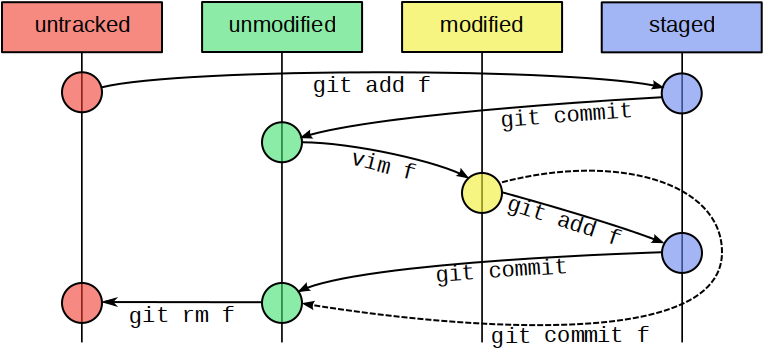
\includegraphics[scale = 0.55]{resources/git_workflow.png}
   \caption{Basic git workflow}
\end{figure}

\subsubsection{One last thing}

Remember when we said that git was a distributed tool that allowed people to collaborate on the same project? We have not covered that part.

Actually, commits can be synchronized with a server. We will not cover it in details at all; for now you just need to now that if your git repository exists on a remote server you can \textbf{push} your tree to make your commits available to other collaborators and \textbf{pull} the latest commits made by other collaborators. The respective commands to perform these two actions are, surprisingly, \texttt{git push} and \texttt{git pull}.

Think of it as a Google doc where you write stuff collaboratively: when you make changes, everybody can see them and when other make changes, you can see them. When you write code as a member of a team, you also want to share your code with your teammates and retrieve code changes from your teammates; most teams do it with git.

\section{Practical exercises}

%You have been created an account and a custom repository on a \href{https://gitea.electrosenpai.dev}{Gitea server}. You will use it to play with git by yourself.
%
%\subsection{Getting access}
%
%\subsubsection{Connection to the platform}
%
%First, visit \href{https://gitea.electrosenpai.dev}{https://gitea.electrosenpai.dev} and login using your email and your password.
%
%Then, change your password. Do not forget it as you will need it to reconnect to the platform in the future.
%
%Verify that you have been given access to a repository (it should be visible on the front page).
%
%\subsubsection{SSH access}
%
%The preferred way to communicate with a git remote (understand \textit{a repository online}) is through SSH. SSH is a protocol providing a secure communication channel between two hosts. It relies on symmetric and asymmetric cryptography.
%
%We are not going to dig into the details of that protocol as it would be out of scope for that tutorial. Instead, remember that we need to generate a private (\textbf{secret}) key and a public \textbf{not secret}) key and to communicate the public key to the git server.
%
%The following command will generate a 4096 bits RSA keypair:
%
%\begin{lstlisting}[language=bash]
%$ssh-keygen -t rsa -b 4096
%Generating public/private rsa key pair.
%Enter file in which to save the key (/home/nicolas/.ssh/id_rsa): # Do not put anything here, it is the right place
%Enter passphrase (empty for no passphrase): 
%Enter same passphrase again:
%Your identification has been saved in /home/nicolas/.ssh/id_rsa.
%Your public key has been saved in /home/nicolas/.ssh/id_rsa.pub.
%The key fingerprint is:
%SHA256:pUuEbId+QRZgIE4Zu7fI/ZqViyISKJDV9nk4f9cLCh4 nicolas@nicolas-laptop
%The key's randomart image is:
%+---[RSA 4096]----+
%|  ++..o.+.       |
%| ooooo =         |
%| oo. .=o+ .      |
%|o  . o=o.+       |
%|o . . .+S    .   |
%|+. + . +E.. o .  |
%|..o o o..+ o . . |
%|o .  = .. .   .  |
%|.. .+.o          |
%+----[SHA256]-----+
%\end{lstlisting}
%
%Following that command, the keys are put in your home, in the hidden folder \texttt{.ssh/}. The public key is the one with the \texttt{.pub} extension. As it is public, it can be shared with anyone without any risk. The private one is the one without extension. You should not touch that file.
%
%Now, copy the content of that public key file (you can use \texttt{cat /home/your\_name/.ssh/id\_rsa.pub} to get it). Then, put it in Gitea: browse \textit{Settings}, \textit{SSH / GPG Keys}, \textit{Manage SSH keys}, \textit{Add key}.
%
%The field \textit{Key name} does not matter. Put the key in \textit{Content}.

\subsection{Git local configuration}

Let us configure git. It should be installed in your machine by now.

\begin{lstlisting}[language=bash]
$git config --global user.name "Firstname Lastname" # Put your own name here and do not forget the quotes!
$git config --global user.email firstname.lastname@mail.com # Put your own name and email here
\end{lstlisting}

The configuration will be saved in your home, in the hidden file \texttt{.gitconfig}. This is where git will look for user configuration, by default. Use \texttt{cat ~/.gitconfig} to see the file content. Confirm that the informations you entered earlier are correct.

\subsection{Try out commands!}

\subsubsection{Cloning the repository}

We are going to use the popular "development platform" \href{https://github.com/}{Github}. This platform is the leader in the industry and millions of developers use it. Most engineering teams use either GitHub or a similar platform on a daily basis.
Create an account there and verificate it by confirming your email.

Then, create a new repository: navigate to \href{https://github.com/new}{https://github.com/new} and write down \texttt{git-tutorial} as the name of the repository. Set the repository visibility to \textbf{Public}.

Once you are done, you should be able to clone the repository in your workstation. Open a terminal and run \texttt{git clone https://github.com/YOUR\_USERNAME\_HERE/git-tutorial.git}. You will be prompted for your Github username and password\footnote{We will not cover SSH access in this tutorial. If you know how to configure it, it is greatly advised to do it!}; enter them and use \texttt{ls}... You should see a new directory there! It is the git repository that you just created.

%You should now be able to clone the repository from Gitea. Go to the repository page and copy its SSH address. Then run \texttt{git clone ADDRESS}.
%
%\begin{lstlisting}[language=bash]
%$git clone ssh://git@gitea.electrosenpai.dev/REPOSITORY_PATH.git
%Cloning into 'git-basics...
%The authenticity of host '[gitea.electrosenpai.dev]:2424 ([IP]:2424)' can't be established.
%ECDSA key fingerprint is SHA256:...
%Are you sure you want to continue connecting (yes/no)? yes
%Warning: Permanently added '[gitea.electrosenpai.dev]:2424,[IP]:2424' (ECDSA) to the list of known hosts.
%remote: Enumerating objects: 3, done.
%remote: Countring objects: 100% (3/3), done.
%remote: Total 3 (delta 0), reused 0 (delta 0)
%Receiving objects: 100% (3/3), done.
%\end{lstlisting}

\begin{lstlisting}[language=bash]
$ls
git-tutorial
$cd git-tutorial
$git status
On branch master

No commits yet

nothing to commit (create/copy files and use "git add" to track)
\end{lstlisting}


\subsubsection{Exercises}

You now have everything you need. We will not work on in-depth exercises as we only covered the basics of git but you now should be able to versionate code and push it to a repository.

You are asked to:

\begin{itemize}
	\item Create a new empty file called \texttt{empty\_file\_1}. Stage it and commit it with a message indicating what the changes are. Repeat this 2 times (name the new files \texttt{empty\_file\_2} and \texttt{empty\_file\_3}).
	\item Create a new file called \texttt{README.md}. Write your name inside. Stage the file and commit it with an appropriate message.
	\item Create a new file called \texttt{modify\_me.txt}. Write \textit{2 + 2 = 5} inside. Stage the file and commit it. Then, edit the file, fix the mistake (\textit{2 + 2 = 4}). Stage those modifications and commit them with an appropriate message.
	\item Push your commits to Github with the command \texttt{git push}.
\end{itemize}

\textbf{Bonus:} put the code from the last section of tutorial 1 in the repository and add features to it. It could be anything, from asking the name of the player and displaying it when he wins, to restricting the number of guesses the player can make. For each feature, make a commit. Do not forget to push when you are done.

At any time, use \texttt{git status} to know what the current status of the repository is. Use \texttt{git log} to see the history of commits.
After a successful push, you can visit the repository page at \href{https://github.com/YOUR\_USERNAME\_HERE/git-tutorial}{https://github.com/YOUR\_USERNAME\_HERE/git-tutorial}. Try it!

\textit{Remember that at any time you can push your commits to the remote. You do not need to do it that the very end. Do it as often as possible.}

\end{document}
